\documentclass{report}
\usepackage[utf8]{inputenc}
\usepackage[T1]{fontenc}
\usepackage{amsmath}
\usepackage{amssymb,amsfonts,textcomp}
\usepackage{array}
\usepackage{hhline}
\usepackage{hyperref}
\hypersetup{colorlinks=true, linkcolor=blue, citecolor=blue, filecolor=blue, urlcolor=blue, pdftitle=, pdfauthor=Gilles Vuidel, pdfsubject=, pdfkeywords=}
\usepackage{graphicx}
\usepackage[top=2.501cm,bottom=2.501cm,left=2.501cm,right=2.501cm,nohead]{geometry}
\usepackage{float}
\usepackage{parskip}
\usepackage{caption}
\usepackage{fancyvrb}
\makeatletter
\newcommand\arraybslash{\let\\\@arraycr}
\makeatother
% centering figures
\makeatletter
\g@addto@macro\@floatboxreset\centering
\makeatother
\setlength\tabcolsep{1mm}
\renewcommand\arraystretch{1.3}

% saut de page après une section
%\let\oldsection\section
%\renewcommand\section{\clearpage\oldsection}

% saut après itemize
\let\EndItemize\enditemize
\def\enditemize{\EndItemize\medskip}

\begin{document}
 \begin{titlepage}
	
	\centering
	
\includegraphics[scale=0.5]{img/logo.png}\\
	
	\bigskip
	\bigskip
	\bigskip	
	{\Huge
		\bfseries
		PixScape 1.2\\
		\bigskip
		User manual\\
	}
	\bigskip
	\bigskip
	\bigskip
	\bigskip
	\bigskip
	
	{\Large		
		Gilles Vuidel, Yohan Sahraoui and Jean-Christophe Foltête\\
		\bigskip
		2019-11-29\\
	}
	
\end{titlepage}

\setcounter{tocdepth}{2}
%\renewcommand\contentsname{}
\tableofcontents

\pagebreak

\chapter{Introduction}

\section{About PixScape}

PixScape software is dedicated to the analysis of the landscape visibility from raster data.
This software integrates the main functionalities available in standard GIS  in this domain and offers other original features such as tangential view and multi-resolution analysis.


\subsection{Authors}
PixScape has been developed at \href{http://thema.univ-fcomte.fr}{ThéMA} laboratory (\href{http://www.univ-fcomte.fr}{Université de Franche-Comté} – \href{http://www.cnrs.fr}{CNRS}) by Gilles Vuidel in collaboration with Jean-Christophe Foltête, Daniel Joly, Yohan Sahraoui et Samy Youssoufi. The PixScape logo has been designed by Xavier Girardet.

\subsection{Terms of use}
PixScape is distributed in open source, under the \href{https://www.gnu.org/licenses/gpl-3.0.html}{GPL} license.\\
Source code can be downloaded from the sourcesup git repository : \url{git://git.renater.fr/pixscape.git}.\\
Users must cite the following reference in their publications :\\
Sahraoui Y., Vuidel G., Joly D, Foltête J-C., 2018. \href{http://dx.doi.org/10.1111/tgis.12457}{Integrated GIS software for computing landscape visibility metrics}, Transactions in GIS, 22 (5), 1310-1323. 


\section{System requirements}

PixScape runs on any computer supporting Java 8 or later (PC under Linux, Windows, Mac, ...). 
However, when dealing with large datasets, the amount of memory (RAM) will limit the maximum area that can be processed. In addition, processing power (CPU) will determine the speed of computing. For details, see section \nameref{perf}.

For GPU computing, PixScape supports only Nvidia graphics card with CUDA. By default, PixScape is compiled with CUDA 6.5. If you cannot install CUDA 6.5, you will need to install the JCuda library corresponding to your CUDA version and launch PixScape in command line (see \nameref{cuda}). JCuda binaries are available here: \href{http://www.jcuda.org/downloads/downloads.html}{www.jcuda.org/downloads/downloads.html}

\section{Installation and launching PixScape}

PixScape is available for downloading at : \url{http://sourcesup.renater.fr/pixscape}.

\begin{itemize}
	\item Download and install Java 8 or later (\href{http://www.java.com}{java.com}). It is best to install 64 bits version of Java.
	\item Download pixscape-1.2.jar
	\item Launch pixscape-1.2.jar
\end{itemize}

PixScape can be used through 2 user interface : the graphical user interface (GUI) and the command line interface (CLI).

The graphical user interface allows to create project, visualize the data, calculate interactively viewsheds and visibility metrics, and perform exhaustive visibility metric calculation on local computer. The command line interface allows to run the same calculations on remote computers as well as on computer clusters.

The following chapter (\ref{gui}) describes all of the software features available from the GUI. Chapter \ref{cli} details how to use PixScape on the command line. Chapter \ref{principles} explains how visibility calculations are implemented in PixScape. The set of available metrics is detailed in Chapter \ref{metrics}. And Chapter \ref{perf} reviews the parallelization modes, performance and memory management.


\chapter{Graphical user interface (GUI)}
\label{gui}

Once PixScape is launched, the first step is to create a project based on a DTM (Digital Terrain Model) covering the studied area.

\section{Project creation}

To create a new project, use the menu File / New project. User must enter a name and a path for the project as well as a DTM in Tiff or AsciiGrid format. \textbf{The coordinate system of the DTM must be projected and in meter unit. If this is not the case, the visibility calculations will be erroneous.} The resolution of the altitudes (Z) can be specified if it is not in meter. For example, if the altitudes are given in centimeter, enter 0.01 in "Z resolution".

\begin{figure}[H]
	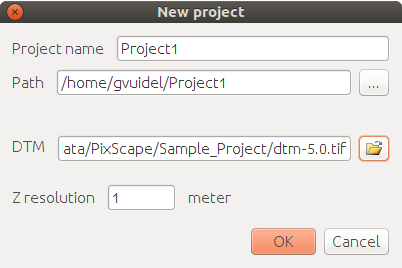
\includegraphics[scale=0.5]{img/new_project-en.png} 
	\caption{Creating a project}
\end{figure}

The created project stores in its folder, the DTM converted in Tiff format with altitudes in meter, and the XML file containing the project settings.
For opening a project, simply select the corresponding XML file from the File / Load Project menu.

The DTM is sufficient to perform visibility calculations, but it can be more interesting to add additional information to perform more accurate analyses.

\section{Data management}

For importing raster data, PixScape supports 2 file formats : Tiff and AsciiGrid.
For Tiff format, the coordinate system can be given by 2 ways : directly in the Tiff file with the GeoTiff extension, or an additional text file with the same name and extension .tfw.


\subsection{Additional layers}
Two additional raster layers can be added to an existing project: the DSM (Digital Surface Model) and the land use.

\subsubsection{DSM}
In PixScape, the DSM corresponds to the height of the object (building, trees, ...) on the ground. The addition of the DTM and the DSM makes it possible to obtain the total elevation of the elements of the landscape. 
The unit of heights must be expressed in meters. To load a DSM, simply select a raster file in Tiff or Asciigrid format from the Data / Load DSM menu. After loading, the DSM is stored in the project directory

\subsubsection{Land use}
The land use layer is used by several landscape configuration metrics (S, IJI, CONTAG, etc.). The codes for land use categories must be between 0 and 255. To load a land use layer, simply select a raster file in Tiff or Asciigrid format from the Data / Load Land Use menu. After loading, the layer is stored in the project directory.

The colors associated with the land use categories are set randomly, but can be changed in the style of the layer. Color changes are automatically saved in the project's XML file to be kept from one opening to the next.

\textbf{These two layers must have exactly the same geometry as the DTM: the same spatial extent and the same resolution.} 

\subsection{Multiscale}
It is possible to add data at coarser resolutions to speed up visibility calculations. This data can be generated directly in PixScape from the Data / Multi scale / Generate menu or imported from the Data / Multi scale / Add scale menu.

\subsubsection{Generate multiscale data}
Generation of a multiscale database can be done directly in PixScape. User must give the required resolutions separated by commas. By default the software proposes 4 resolutions separated by a factor of 3. If the resolution of the initial data is 1 meters, the software will propose the resolutions 3m, 9m, 27m and 81m.

\begin{figure}[H]
	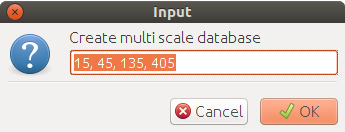
\includegraphics[scale=0.5]{img/gen_ms-en.png} 
	\caption{Multiscale database generation}
\end{figure}

It is recommended to use resolutions that follow a geometric sequence of a factor 2, 3 or 4.
PixScape will create a new DTM for each resolution, as well as the DSM and land use if these layers are present in the project.
For the DTM and the DSM the pixels are aggregated by the arithmetic mean, for the land use, the pixels are aggregated by the mode \ textit {ie.} the dominant land use category.
At the end of the processing, all the new layers are saved in Tiff format in the project directory and are added in the layer tree of the main window.


\subsubsection{Import data}
The multiscale database can be imported for each scale. At least DTM must be provided, and DSM plus landuse should be provided if these layers are already presents for the initial scale. As with the creation of the project, the resolution of the altitudes of the DTM can be indicated.

\begin{figure}[H]
	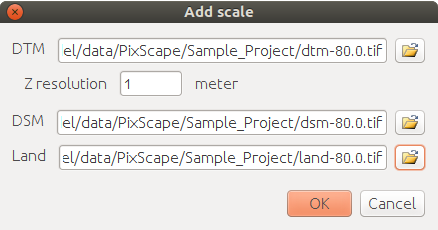
\includegraphics[scale=0.5]{img/add_scale-en.png} 
	\caption{Import layers for one scale}
\end{figure}

The resolution of the DSM heights must be in meters and the land use codes must be between 0 and 255. For land use, codes may vary from one scale to another to differentiate objects that do not have the same meaning according to the resolution, for example a tree and a forest, a building and a village.
The three layers must have exactly the same geometry: the same spatial extent and the same resolution.
Finally, the spatial extent must cover at least the spatial extent of the initial data.

When the project contains multiscale data, it can be used in visibility calculations by activating the multiscale setting in the Options window (see \nameref{options}).


\section{Visibility calculation}

Two visibility calculation methods are available from the Visibility menu: the viewshed and the tangential view.
For each method, the user can view the result for a given observation point by clicking on the map.

\subsection{Viewshed}
The viewshed corresponds to the surface on the plane (x, y) containing the set of points visible from the observation point O.

\begin{figure}[H]
	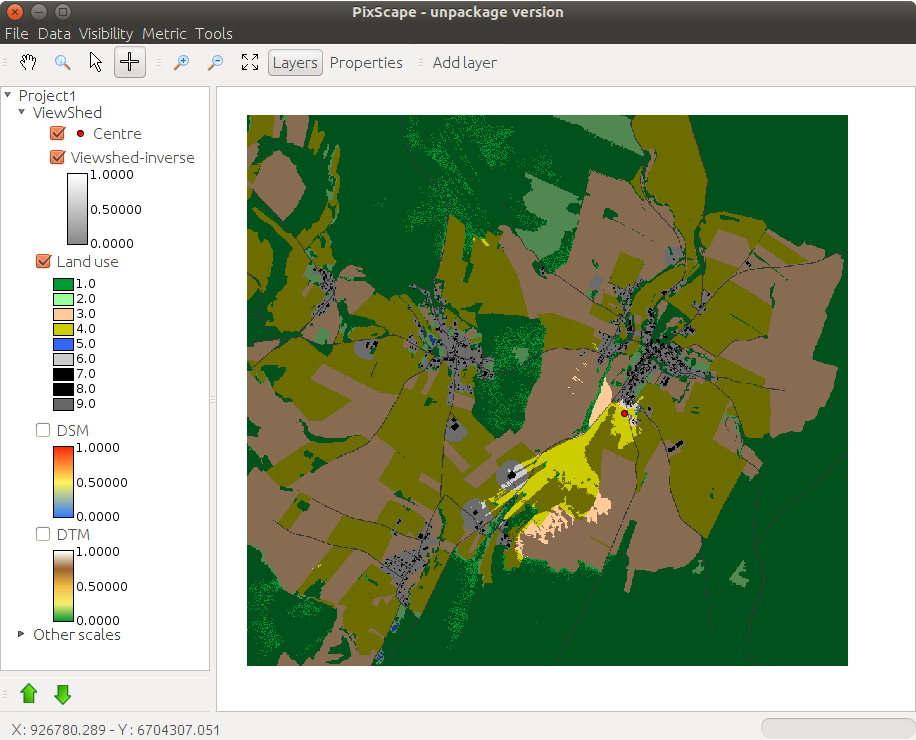
\includegraphics[scale=0.5]{img/viewshed-en.png} 
	\caption{Resulting viewshed from the red point. The viewshed is displayed by transparency.}
	\label{viewshed}
\end{figure}

The calculation of a viewshed can be accessed from the Visibility / Viewshed menu. A window appears showing all the parameters that are relevant for the calculation of a viewshed (figure \ref{viewshed_param_fig}).

\begin{figure}[H]
	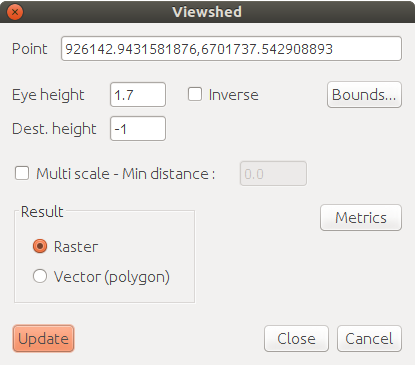
\includegraphics[scale=0.5]{img/viewshed_dlg-en.png} 
	\caption{Viewshed settings window}
	\label{viewshed_param_fig}
\end{figure}

\subsubsection{Parameters}
\label{viewshed_param}
\begin{itemize}
	\item Point: coordinates of the observation or observed point O. It can be entered manually or given by clicking on the map.
	\item Eye height (h1): height in meter of the observer eye
	\item Dest. height (h2): height in meters of observed point(s). If set to -1, the height of the DSM is used. If the project does not contain a DSM, the height is zero.
	\item Inverse: unchecked by default, point O is the observation point \textit{ie.} the eye of the observer (figure \ref{height_view}). The viewshed corresponds to all the points visible from O. Conversely, if the box is checked, the point O becomes the observed point (figure \ref{height_view_inverse}). The viewshed then corresponds to the set of points from which the observer sees the point O.
	\item Bounds: this window allows you to restrict the eyesight of the observer in the 3 dimensions (see \nameref{bounds})
	\item Multiscale: enables or disables multiscale calculation. If enabled, the minimal distance in meter before the change of scale must be entered.
\end{itemize}


\begin{figure}[H]
	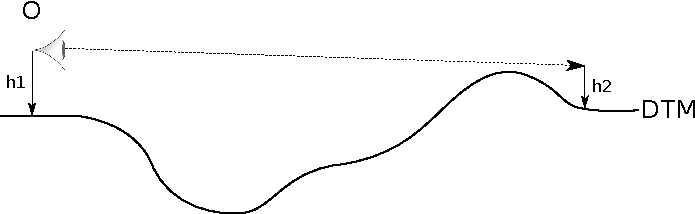
\includegraphics{img/height_view-en.pdf} 
	\caption{Default mode: O is the observation point, h1 is the height of the eye and h2 is the destination height or the DSM height if Dest. height = -1}
	\label{height_view}
\end{figure}

Dest. height (h2) parameter is often used with inverse mode to analyze the impact of a construction (pylon, wind turbine, etc). The resulting viewshed then corresponds to the set of points from which the new construction of a height h2 will be visible (figure \ref{height_view_inverse}).

\begin{figure}[H]
	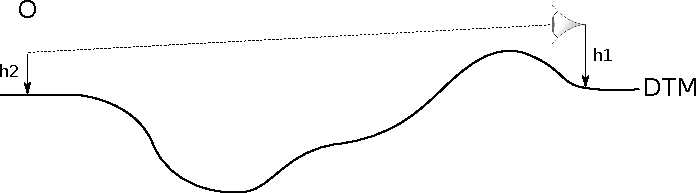
\includegraphics{img/height_view_inverse-en.pdf} 
	\caption{Inverse mode: O is the observed point, h1 is the height of the eye and h2 is the destination height (defined by  Dest. height or the DSM height if Dest. height = -1)}
	\label{height_view_inverse}	
\end{figure}

\subsubsection{Results}

The viewshed can be displayed on the map in raster or vector form according to the choice made in the Result panel. In raster, the bright areas correspond to the visible areas. Conversely, in vectorial, the dark areas correspond to the visible areas. In both cases, the result layer can be exported by right clicking on the layer.

Metrics can be selected from the Metrics button to be calculated on the current viewshed. For more information on metrics, see the section \nameref{metrics}.

\begin{figure}[H]
	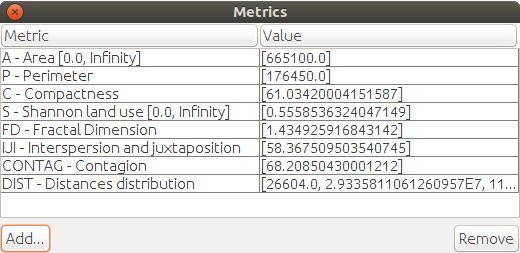
\includegraphics[scale=0.5]{img/viewshed_metric-en.png} 
	\caption{Metrics calculated from the current viewshed}
	\label{viewshed_metric}
\end{figure}

After modifying a parameter, simply click on the Update button to update the viewshed on the map as well as the metrics if they are displayed.


\subsection{Tangential view}

The calculation of a tangential view can be accessed from the Visibility / Tangential View menu. A window appears showing the settings for the calculation of the view as well as for displaying the result (figure \ref{viewtan_param}). 

\begin{figure}[H]
	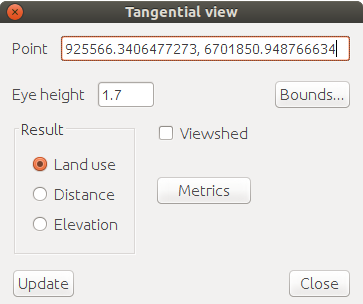
\includegraphics[scale=0.5]{img/viewtan_dlg-en.png} 
	\caption{Tangential view settings}
	\label{viewtan_param}
\end{figure}

\subsubsection{Parameters}

\begin{itemize}
	\item Point: coordinates of the observation or observed point O. It can be entered manually or given by clicking on the map.
	\item Eye height (h1): height in meter of the observer eye
	\item Bounds: this window allows you to restrict the eyesight of the observer in the 3 dimensions (see \nameref{bounds})
	\item Viewshed: if checked, the viewshed is displayed on the map.
	\item Result: choice of the result displayed (see \nameref{viewtan_result}).
\end{itemize}

The angular resolution parameter and the use of the multiscale database cannot be set in this window but only on the Options window (see \nameref{options}).

\subsubsection{Results}
\label{viewtan_result}
The result is displayed in a new window representing the tangential view (figure \ref{viewtan_land}). The coordinates of this image are in degrees from -180° to + 180° horizontally and -90° to + 90° vertically, the north being at 0° in the middle of the image.

\begin{figure}[H]
	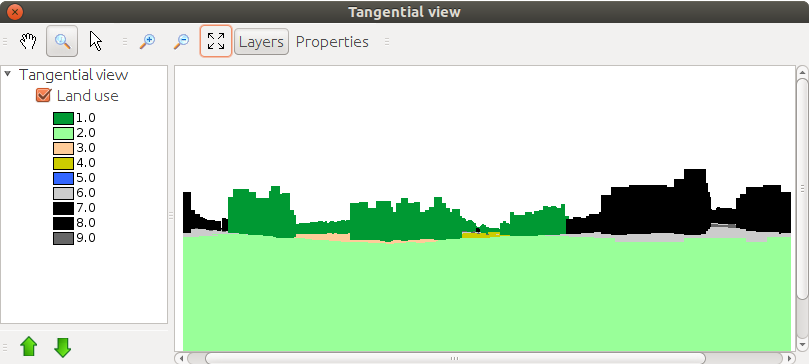
\includegraphics[scale=0.5]{img/viewtan_land-en.png} 
	\caption{Tangential view. The colors represent the land use.}
	\label{viewtan_land}
\end{figure}

By default, colors represent the land use categories (figure \ref{viewtan_land}). By selecting Distance in the result panel, the tangential view displays the distances to the observation point (figure \ref{viewtan_dist}).

\begin{figure}[H]
	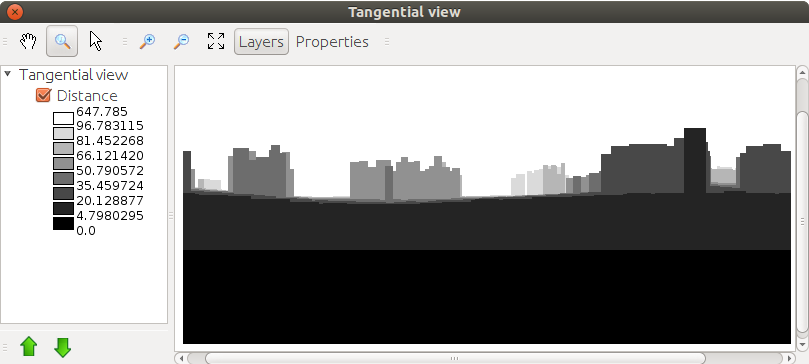
\includegraphics[scale=0.5]{img/viewtan_dist-en.png} 
	\caption{Tangential view. The colors represent the distance to the observation point.}
	\label{viewtan_dist}
\end{figure}

Metrics can be selected from the Metrics button to be calculated on the current view. For more information on metrics, see the section \nameref{metrics}.

After modifying a parameter, simply click on the Update button to update the view as well as the metrics if they are displayed.


\subsection{Multi-viewshed}
\label{multi_viewshed}
The Visibility / Multi Viewshed menu allows you to calculate several viewsheds from a shapefile containing observation points.

\begin{figure}[H]
	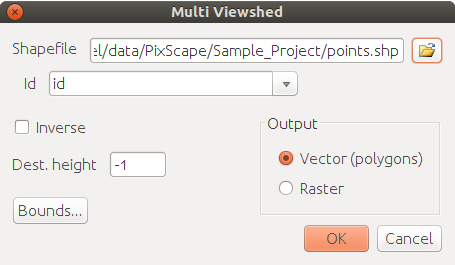
\includegraphics[scale=0.5]{img/multi_viewshed-en.png} 
	\caption{Multi-viewshed settings}
	\label{multi_viewshed_dlg}
\end{figure}

\subsubsection{Parameters}

\begin{itemize}
	\item Shapefile : shapefile containing observation points.
	\item Id : shapefile attribute used as identifier. This parameter is useful only for vectorial result.
	\item Inverse: unchecked by default, the shapefile points represent the observation points \textit{ie.} the eye of the observer. Conversely, if the box is checked, the shapefile points becomes the observed points. For details see the viewshed \nameref{viewshed_param}.
	\item Dest. height (h2): height in meters of observed point(s). If set to -1, the height of the DSM is used. If the project does not contain a DSM, the height is zero.
	\item Bounds: this window allows you to restrict the eyesight of the observer in the 3 dimensions for all observation points (see \nameref{bounds}). If the shapefile contains the attributes (dmin, dmax, zmin, zmax, orien et amp), they will be used in place of these settings.
	\item Output : format of the result layer : vector or raster.
	\item Raster : for raster output, the result may be the number of visible points (count), the total visible area (angular area) or the total visible height(angular height).
\end{itemize}

The eye height (h1) parameter and the use of the multiscale database cannot be set in this window but only on the Options window (see \nameref{options}).

\subsubsection{Result}
The resulting viewsheds can be displayed on the map in raster or vector format according to the selected option on Output panel. In both cases, the result layer is saved in the project directory.

In vector, the layer contains a multi-polygon for each viewshed (figure \ref{multi_viewshed_vector}). Each multi-polygon has an Id attribute allowing to link the shape with the corresponding observation point.

\begin{figure}[H]
	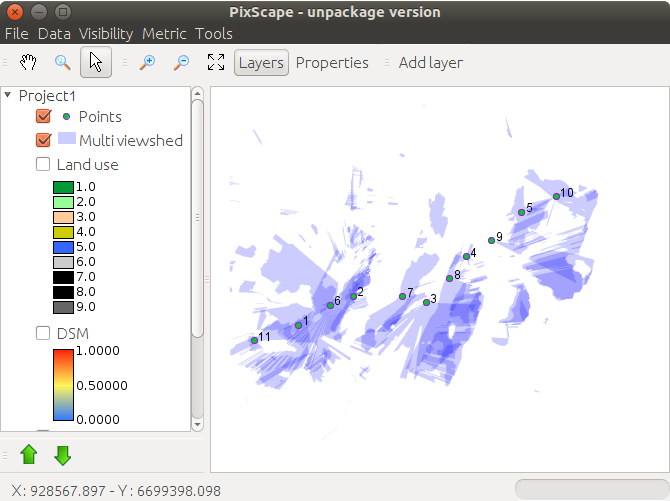
\includegraphics[scale=0.5]{img/multi_viewshed_vector-en.png} 
	\caption{Multi-viewshed in vector format}
	\label{multi_viewshed_vector}
\end{figure}

In raster, the value of the pixel corresponds to the number of times the pixel is contained in a viewshed \textit{ie.} the number of observation points seeing the pixel or, in inverse mode, the number of observation points seen from the pixel (figure \ref{multi_viewshed_raster}). 
If "angular area" or "angular height" is selected, the pixel value is the total area or height in degree (figure \ref{multi_viewshed_raster_deg}).

\begin{figure}[H]
	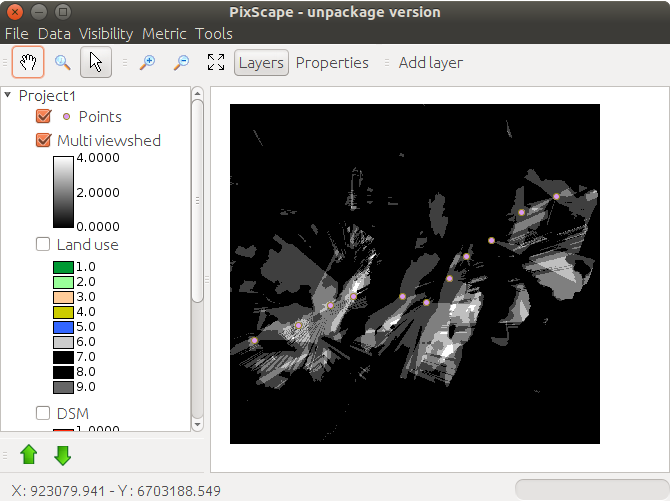
\includegraphics[scale=0.5]{img/multi_viewshed_raster-en.png} 
	\caption{Multi-viewshed in raster format - Dest. height (h2) = -1 - count option}
	\label{multi_viewshed_raster}
\end{figure}

\begin{figure}[H]
	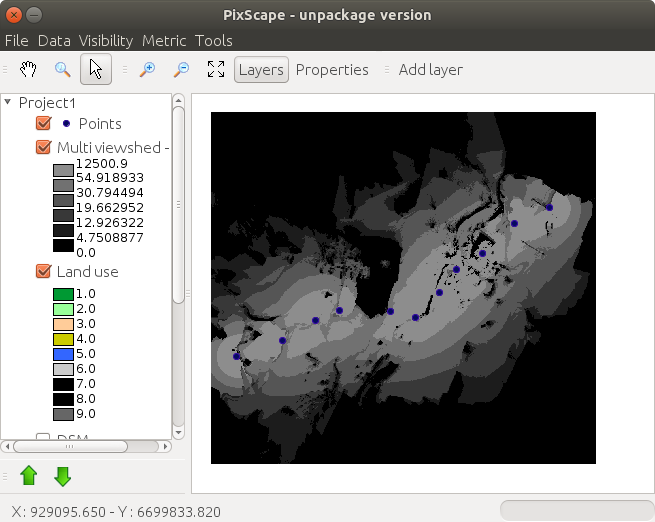
\includegraphics[scale=0.5]{img/multi_viewshed_raster_deg-en.png} 
	\caption{Multi-viewshed in raster format - Dest. height (h2) = 200 - angular area option}
	\label{multi_viewshed_raster_deg}
\end{figure}

\subsection{Eyesight bounds}
\label{bounds_ui}
For all visibility calculations into PixScape, the eyesight can be restricted in all 3 dimensions. Details are described in the section \nameref{bounds}.

These bounds can be set from the Bounds window (figure \ref{bounds_dlg}). When the observation points come from a shapefile, the setting of the eyesight can be differentiated for each point by adding the 6 parameters (dmin, dmax, zmin, zmax, orien, amp) in the shapefile attributes table. The "Set point attributes" menu allows you to automatically add them to an existing shapefile (see \nameref{add_attributes}).

\begin{figure}[H]
	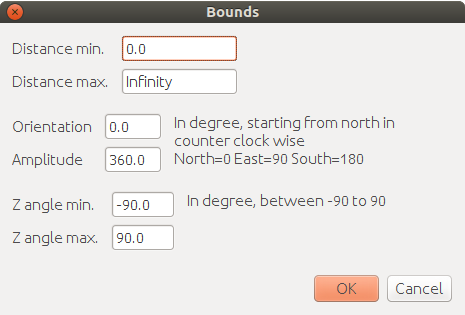
\includegraphics[scale=0.5]{img/bounds-en.png} 
	\caption{Settings of the eyesight. By default the eyesight bounds are unlimited.}
	\label{bounds_dlg}
\end{figure}

\section{Visibility metric calculation}
\label{calc_metrics}
PixScape can agregate the result of a viewshed or tangential view by several indicators, or metrics. The available metrics are detailed in the chapter \nameref{metrics}.

The Visibility menu already allows you to calculate several metrics on the current view. But this "manual" operation is only possible for a few observation points.

The Metric menu allows you to launch a visibility calculation (planimetric or tangential) and the calculation of the metrics for a set of observation points in a single execution.


\begin{figure}[H]
	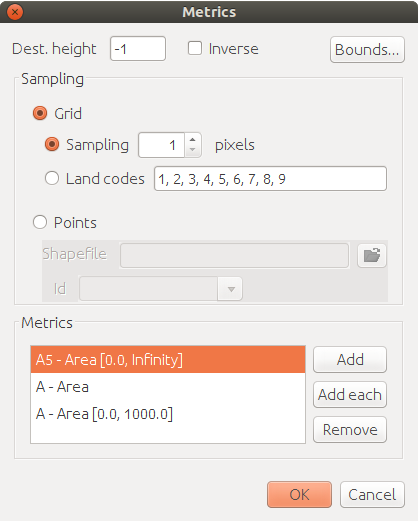
\includegraphics[scale=0.5]{img/metrics-en.png} 
	\caption{Settings for metrics calculation}
	\label{metrics_dlg}
\end{figure}

\subsection{View parameters}
View-specific parameters are displayed at the top of the window (figure \ref{metrics_dlg}) and depend on the type of view selected in the Metric menu: planimetric (for viewshed) or tangential.

\begin{itemize}
	\item Inverse (planimetric only): unchecked by default, the shapefile points represent the observation points \textit{ie.} the eye of the observer. Conversely, if the box is checked, the shapefile points becomes the observed points. For details see the viewshed \nameref{viewshed_param}.
	\item Dest. height (h2) (planimetric only): height in meters of observed point(s). If set to -1, the height of the DSM is used. If the project does not contain a DSM, the height is zero.
	\item Bounds: this window allows you to restrict the eyesight of the observer in the 3 dimensions for all observation points (see \nameref{bounds}). If the selected sampling is Points and the shapefile contains the attributes (dmin, dmax, zmin, zmax, orien et amp), they will be used in place of these settings.	
\end{itemize}

The other parameters for the view (\textit {eg.} eye height, angular resolution, ...) must be set before in the Options window (see \nameref{options}).


\subsection{Sampling}
\label{sampling}
Observation points can be given in raster (Grid option) or vector (Points option). The format of the result (raster or vector) is related to the type chosen.

\subsubsection{Grid sampling (raster)}
With grid option, the sampling of the observation points is done from the grid of the DTM at the finest resolution. Two options are possible: regular sampling on the grid or land use category.

By default, the sampling is regular and set at 1 pixel, which corresponds to an exhaustive run of the set of pixels of the image \textit{ie.} a visibility calculation will be executed from each pixel. If we increase the sampling to 3, only one pixel out of 3 will be used in each dimension, so we will compute a view only for 1 pixel out of 9 of the grid (figure \ref{grid_sampling}).

\begin{figure}[H]
	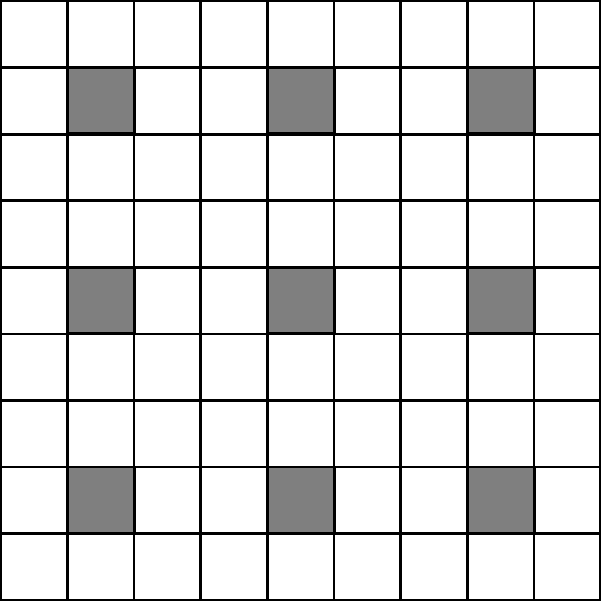
\includegraphics[scale=0.5]{img/grid_sampling.pdf} 
	\caption{Grid sampling every 3 pixels on each dimension. 9 views will be calculated from the 9 shaded pixels.}
	\label{grid_sampling}
\end{figure}

If the sampling is done by land use category, the views will be calculated only from the pixels belonging to one of the listed categories. Land use codes must be separated by commas.

The result will be one or more raster layers. It will contain one layer for each metric and for each distance range defined in the metric setting.


\subsubsection{Points sampling (vector)}
Instead of using the raster grid sampling, you can provide a set of points from a shapefile.

The result will be in the form of a point layer corresponding to the input shapefile. The result of the metrics will be stored in the attribute table of the shapefile.


\subsection{Metric parameters}
\label{param_metrics}
For each observation point, a set of metrics can be computed. The Metrics panel allows you to select them and to set distances and landuse categories if needed. The same metric can be added several times with different settings.

\begin{figure}[H]
	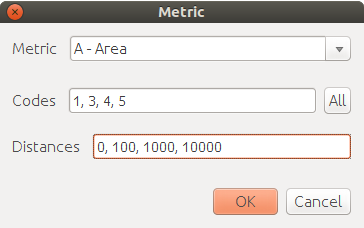
\includegraphics[scale=0.5]{img/metric_param-en.png} 
	\caption{Parameters of metric A}
	\label{metric_param_dlg}
\end{figure}

Figure \ref{metric_param_dlg} shows the settings of the metric A. In this example, metric A will only be calculated on the landuse classes 1, 3, 4 and 5 for 3 distance intervals [0-100[ , [100-1000[ and [1000-10000[. The result will contain 3 values for each observation point, one for each distance interval.

"Add each" button adds the selected metric several times: one for each land-use category.

Several landuse categories can be grouped in one class with the dash character "-" (figure \ref{metric_param_group_dlg}). This makes it possible to keep a detailed land-use and at the same time carry out some analysis on more general classes.

\begin{figure}[H]
	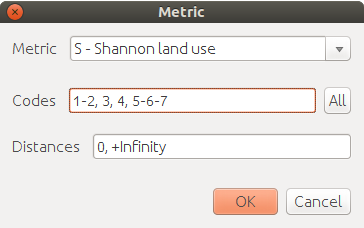
\includegraphics[scale=0.5]{img/metric_param_group-en.png} 
	\caption{Parameters of metric S. Land-use category are grouped in 4 classes.}
	\label{metric_param_group_dlg}
\end{figure}

The grouping of land-use categories is not useful for metric A. Indeed, this metric does not differentiate the categories in each class. For example, \verb|1,3,4,5| and \verb|1-3,4-5| will give the same result for the metric A.

\subsection{Results}

The result of the calculation of metrics is displayed on the map by one or more layers in raster or vector format depending on the input format used for sampling. Each layer can be exported by right clicking on the layer name and the "Export ..." menu.

\subsubsection{Raster}
For raster, the result is a set of raster layers, one for each metric and each distance interval. Each layer can be exported in Tiff or AsciiGrid format.

For the settings of the figure \ref{metric_param_dlg}, PixScape adds 3 raster layers (figure \ref{metric_result_rast}) for the 3 distance intervals.

If the sampling is greater than 1, the pixel size is increased proportionately as the sampling factor. 

\begin{figure}[H]
	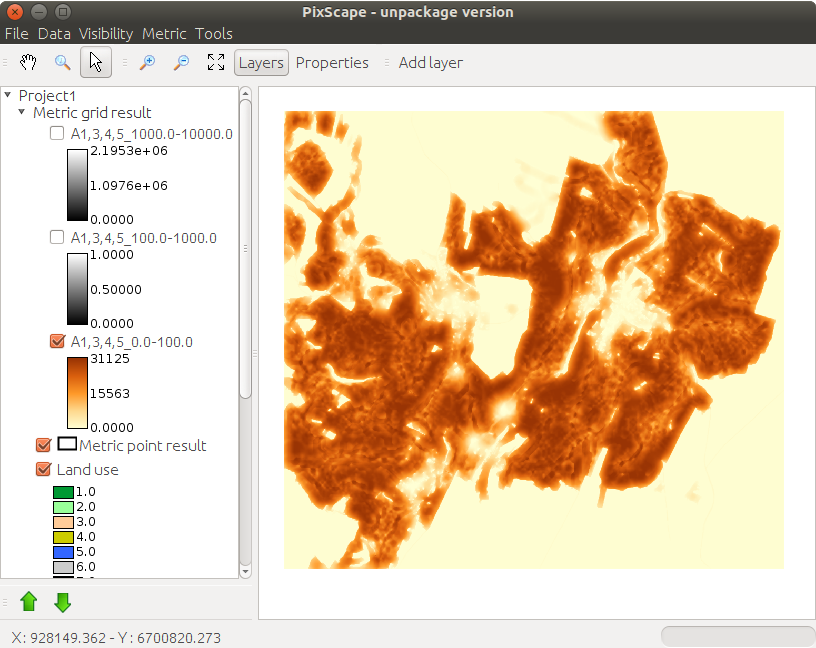
\includegraphics[scale=0.5]{img/metric_result_rast-en.png} 
	\caption{Metric result with grid sampling.}
	\label{metric_result_rast}
\end{figure}

\subsubsection{Vector}

In vector, the result is a point layer containing the metrics values in the attribute table (figure \ref{metric_result_attr}). By default the first metric is displayed with proportional circle (figure \ref{metric_result_vect}). To display another metric, simply change the attribute selected in the "Circle" tab of the layer style window.

\begin{figure}[H]
	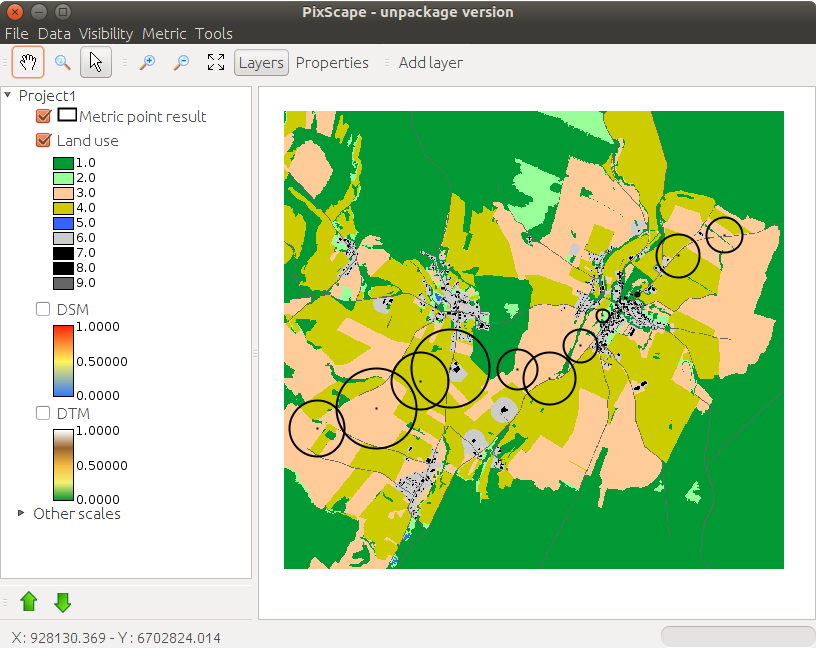
\includegraphics[scale=0.5]{img/metric_result_vect-en.png} 
	\caption{Metric result from a point layer. The first metric is displayed by circles proportional to the value of the metric.}
	\label{metric_result_vect}
\end{figure}

The layer "Metric point result" can be exported in shapefile or text format by right clicking on the layers name and the menu "Export ...".

\begin{figure}[H]
	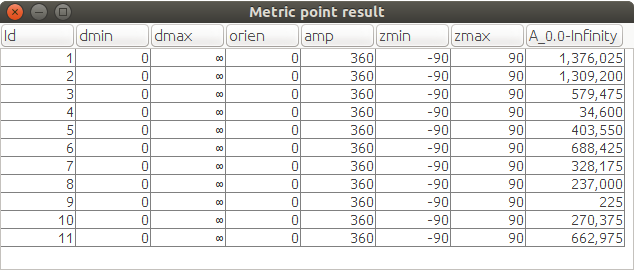
\includegraphics[scale=0.5]{img/metric_result_attr-en.png} 
	\caption{Attribute layer of the result layer.}
	\label{metric_result_attr}
\end{figure}

The attribute table of the result layer is accessible by right clicking on the layer name and the "Attribute table" menu. It contains, in addition to the metrics, the 6 parameters used for limiting the eyesight, allowing to keep these parameters with the results.

\section{Tools and options}
\label{tools}

\subsection{Add eyesight attributes}
\label{add_attributes}
For all visibility calculations, the eyesight can be restricted by the Bounds window (figure \ref{bounds_dlg}). This solution is useful if each observation point has the same limitations of the eyesight.
The Tools / Set point attributes menu is useful for specifying different restrictions for each observation point. This function adds the 6 attributes to a shapefile with the default values defined by the Bounds window. You can then with your favorite GIS modify the restriction values for each observation point.
The output shapefile can be used for calculation of metrics (\ref{calc_metrics}) or multi viewshed (\ref{multi_viewshed}).

\begin{figure}[H]
	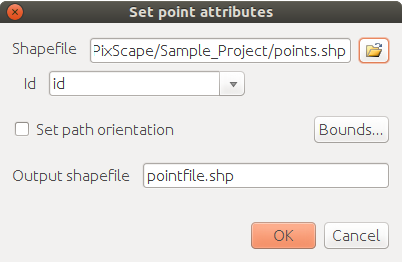
\includegraphics[scale=0.5]{img/add_attributes-en.png} 
	\caption{Add eyesight bound attributes to a shapefile}
	\label{add_attributes_dlg}
\end{figure}

\subsubsection{Eyesight along a path}
The check box "Set path orientation" calculates  the orientation of each point depending on the next one. When this option is checked, the orientation parameter of the "Bounds" window is ignored and each point may have an different orientation.

\begin{figure}[H]
	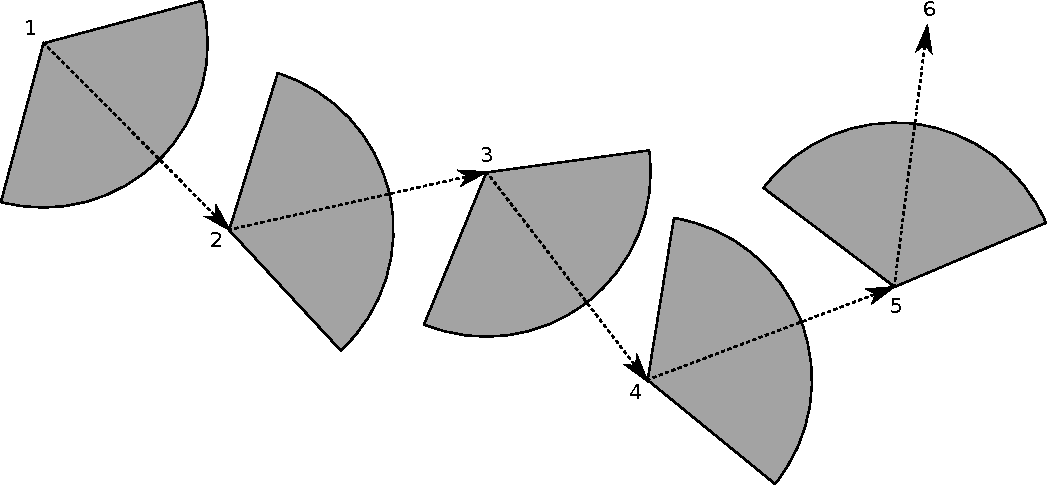
\includegraphics[scale=0.8]{img/path_orien.pdf} 
	\caption{Eyesights along a path. The orientation is calculated by the next point. The amplitude is constant.}
	\label{path_orien}
\end{figure}

The points order is defined by "id" attribute which is sorted with natural ordering.
This option is useful only with an amplitude less than 360°.


\subsection{Options}
\label{options}
The general project options are available from the Tools / Options menu.
These options are saved automatically in the xml file of the project. They are used for all the visibility calculations except when an option is also present in the settings window of a processing. For example, the height of the eye can be changed directly in the settings window of a planimetric or tangential view, but it is not available for calculating metrics. In the latter case, the height of the observer's eye will be set from the general options window.

\begin{figure}[H]
	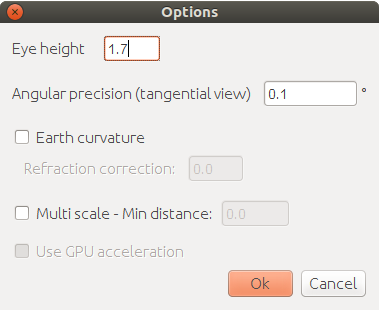
\includegraphics[scale=0.5]{img/options-en.png} 
	\caption{General options}
\end{figure}

\subsubsection{Height of the observer's eye}
Eye height parameter ($h1$) sets the hieght of the observer from the DEM. The height is in meters. For more details, see \nameref{principles} and the figure \ref{ray_side}.

\subsubsection{Angular precision}
Angular precision parameter ($\alpha$) sets the resolution in degrees of the tangential view. It is set by default to 0.1°, which corresponds to 3600 rays if the amplitude of the view is 360 °. For more details, see \nameref{principles_tan} and the figure \ref{grid_tan}.

\subsubsection{Earth curvature}
\label{curvature}
The visibility calculations in PixScape can take into account the curvature of the Earth, which can play a role in the case of a view greater than several tens of kilometers. The principle of computation is simple: the more the distance to the observer increases, the more the height of the visible objects diminish.
The height taking into account the curvature of the Earth $z'_i$ of a point $i$ is calculated as follows:

$$z'_i = z_i - \frac{d_i^2}{D}$$

with $z_i$ the elevation of the DTM at point $i$, $d_i$ the distance between the point $i$ and the observer and $D$ the Earth diameter (12 740 000 meters).

The Earth curvature may be compensated by the light refraction in the atmosphere.
In PixScape, when the Earth curvature is taken into account, the refraction parameter can be specified. It is set to 0.13 by default. The calculation of the height becomes

$$z'_i = z_i - (1-\rho)\frac{d_i^2}{D}$$

with $\rho$ the refraction coefficient between 0 and 1. If $\rho=0$, we return to the preceding formula without refraction.


\subsubsection{Multiscale}
When the project contains data with several resolutions, the visibility calculations can be done in multiscale by activating this option. The minimum distance parameter must be defined. It ensures a minimum distance in meters before changing resolution.

For more details on the multiscale calculations, see \nameref{multires}.


\subsubsection{GPU acceleration}
This parameter is used to perform visibility calculations on the graphics card processor (GPU) instead of the central processor. Runtime gains can be significant for Nvidia Tesla graphics cards, designed for high-performance computing (see \nameref {perf}). On the other hand, not all metrics are optimized for the GPU. Metrics A and S are the only ones to be optimized. If you use other metrics, the time savings will be minimal or non-existent.

The parameter is disabled if PixScape can not use GPU acceleration. The causes can be multiple: no NVidia graphics card, no CUDA support, not the right version of CUDA (6.5).

GPU acceleration cannot be used for multiscale calculations. If multiscale option is enabled, GPU acceleration will not be used even if it is enabled.


\chapter{Command line interface (CLI)}
\label{cli}
Once a project has been created from the GUI, it is possible to use PixScape on the command line. This mode is useful for running the software on a remote computer without a graphical interface, automatically launching several processes, or submitting executions on a cluster.

\section{Starting}

\subsection{Launch PixScape in CLI mode}
First you have to open a terminal window. Then, go to the directory of the Graphab program with \textit{cd} command. Finally, type the following command to display the PixScape help screen :
\begin{Verbatim}
java -jar pixscape.jar --help
\end{Verbatim}
Result
\begin{Verbatim}
Usage :
java -jar pixscape.jar --metrics
...
...
\end{Verbatim}
You’re ready to use PixScape in CLI mode.

\subsection{Syntax}
\subsubsection{Definition}
Commands always start with a double dash: \verb|--project, --metrics, ...|\\
Global options start with only one dash: \verb|-proc, -bounds, ...|\\
Parameters does not have dash: \verb|dmin, inverse, ...|

\subsubsection{Character separator}
Blank spaces are used to separate commands and parameters.  You cannot have a name containing blank spaces.

\subsubsection{Help screen syntax}
In the help screen, elements enclosed in brackets are optional. Therefore, elements not in brackets are mandatory. The character \verb+|+ separates the possible options.

\section{Commands}

\subsection{--help : show help screen}
Command:
\begin{Verbatim}
java -jar pixscape-1.2.jar --help
\end{Verbatim}
Result:
\begin{Verbatim}
Usage :
java -jar pixscape.jar --metrics
java -jar pixscape.jar [-mpi | -proc n | -cuda n]
--project project_file.xml
[--landmod zone=filezones.shp id=fieldname code=fieldname dsm=file.tif [selid=id1,...,idn]]
[-zeye val] [-zdest val] [-resdir path]
[-bounds [dmin=val] [dmax=val] [orien=val] [amp=val] [zmin=val] [zmax=val]]
[-sampling n=val | land=code1,..,coden | points=pointfile.shp id=fieldname]
[-multi dmin=val | -mono]
[-earth flat|curved [refrac=val]]
commands

Commands list :
--viewshed [inverse] x y [resfile=raster.tif]
--viewtan [prec=deg] x y [resname=name]
--multiviewshed format=vector|raster [inverse] [degree=area|height] [resname=name]
--planmetric [inverse] metric1[[code1,...,coden]][_d1,...,dm] ... metricn[[code1,...,coden]][_d1,...,dm]
--tanmetric [prec=deg] metric1[[code1,...,coden]][_d1,...,dm] ... metricn[[code1,...,coden]][_d1,...,dm]
--toobject [degree=area|height] [agreg=eye|object] objects=pointfile.shp id=fieldname [resname=name]
\end{Verbatim}

\subsection{--metrics : show metrics}
This command lists all available metrics with their short name and full name.

Commande :
\begin{Verbatim}
java -jar pixscape-1.2.jar --metrics
\end{Verbatim}
Résultat :
\begin{Verbatim}
===== Metrics =====
A - Area
S - Shannon land use
P - Perimeter
C - Compactness
FD - Fractal Dimension
AG - Aggregation index
CONTAG - Contagion
ED - Edge Density
PD - Patch Density
PMS - Patch Mean Size
DIST - Distances distribution
SL - Skyline ratio
SD - Shannon depth
DL - Depth line
\end{Verbatim}

\subsection{--project : load project}
This command sets the path to the project xml file.
\begin{Verbatim}[commandchars=\\\{\}]
java -jar pixscape-1.2.jar --project \textit{path2myproject/myproject.xml}
\end{Verbatim}
This command loads the project \textit{myproject} contained in the \textit{path2myproject} folder.

The \verb|--project| command can be used only once and must be the first command.  All of the following commands below require a loaded project

\subsection{--landmod : land use changes}

\begin{Verbatim}[commandchars=\\\{\}]
--landmod zone=\textit{filezones.shp} id=\textit{fieldname} code=\textit{fieldname} dsm=\textit{file.tif} [selid=\textit{id1,...,idn}]
\end{Verbatim}

\subsubsection{Required parameters}
\begin{itemize}
	\item \verb|zone=filezones.shp| : polygon shapefile containing land use changes.
	\item \verb|id=fieldname| : field name of the shapefile used for identifying polygons. If values are not unique, polygons with the same identifier will be applied in a single change.
	\item \verb|code=fieldname| : field name of the shapefile storing the new land use category of the polygon.
	\item \verb|dsm=file.tif| : raster storing the new values of the DSM used for each land use change. The geometry of the raster must be exactly the same as the project DEM.
\end{itemize}

\subsubsection{Optional parameter}
\begin{itemize}
	\item \verb|selid=id1,...,idn| : list of polygon identifiers to process. If this parameter is not set, all polygons of the shapefile are processed.
\end{itemize}

\subsubsection{Description}
This command must be placed before the visibility calculation commands. It will duplicate the project for each polygon of the shapefile and change the landuse covered by the polygon and the DSM. The commands following this one, will be executed on each modified project.

The newly created projects will be named by the identifier of the polygon(s) and stored in the project directory.

\subsection{--viewshed : planimetric view or viewshed}
\begin{Verbatim}[commandchars=\\\{\}]
--viewshed [inverse] \textit{x} \textit{y} [resfile=\textit{raster.tif}]
\end{Verbatim}

\subsubsection{Required parameters}
\begin{itemize}
	\item \verb|x| : abscissa of the observation point in the coordinate system of the DTM
	\item \verb|y| : ordinate of the observation point in the coordinate system of the DTM
\end{itemize}

\subsubsection{Optional parameters}
\begin{itemize}
	\item \verb|inverse| : reverse mode, the point O becomes the observed point
	\item \verb|resfile=raster.tif| : allow to specify another name for the file storing the result
\end{itemize}

\subsubsection{Description}
The \verb|--viewshed| command allows to calculate the viewshed from an observation point.
The result is stored in a raster file of the same size as the DTM in Tiff format. 
In this raster, all pixels set to 1 represents the viewshed, other pixels are set to 0.

\subsubsection{Examples}
The example below calculates the viewshed for an observer located at the point (925560, 6702495). The result is stored in the projet folder in a file named : \verb|viewshed-925560,6702495.tif|.
\begin{Verbatim}
	--viewshed 925560 6702495
\end{Verbatim}

This second example calculates the viewshed in reverse mode (ie. the given coordinates represent the observed point) and stored the result in the file \verb|bassin1.tif|.
\begin{Verbatim}
	--viewshed inverse 925560 6702495 resfile=bassin1.tif
\end{Verbatim}

\subsection{--viewtan : tangential view}
\begin{Verbatim}[commandchars=\\\{\}]
--viewtan [prec=\textit{deg}] \textit{x} \textit{y} [resname=\textit{name}]
\end{Verbatim}

\subsubsection{Required parameters}
\begin{itemize}
	\item \verb|x| : abscissa of the observation point in the coordinate system of the DTM
	\item \verb|y| : ordinate of the observation point in the coordinate system of the DTM
\end{itemize}

\subsubsection{Optional parameters}
\begin{itemize}
	\item \verb|prec=deg| : angular precision in degrees. If this parameter is not set, the angular precision stored in the project will be used.
	\item \verb|resname=name| : allow to specify another name for the files storing the result
\end{itemize}

\subsubsection{Description}
The \verb|--viewtan| command allows to calculate the tangential view from an observation point. Results are stored in 2 or 3 raster files in Tiff format depending on whether the project contains a land use layer.
\begin{itemize}
	\item \verb|elev| : elevation of the DTM
	\item \verb|dist| : 2D distance from the observation point
	\item \verb|land| : land use, if present in the project
\end{itemize}

The rasters size depends on the angular precision. For a precision of 0.1° and an amplitude of 360°, the rasters size will be 3600x1800 pixels. Their coordinate system unit is set in degrees.

\subsubsection{Examples}
The example below calculates the tangential view for an observer located at the point (925560, 6702495). The result is stored in the projet folder in a files named: \verb|viewtan-925560,6702495-elev.tif|, \verb|viewtan-925560,6702495-dist.tif| and \verb|viewtan-925560,6702495-land.tif| if the project contains a land use layer.
\begin{Verbatim}
	--viewtan 925560 6702495
\end{Verbatim}

The second example calculates the tangential view with an angular precision of 0.05° and stored the result in the files \verb|view1-elev.tif|, \verb|view1-dist.tif| and \verb|view1-land.tif| if the project contains a land use layer.
\begin{Verbatim}
	--viewtan prec=0.05 925560 6702495 resname=view1
\end{Verbatim}


\subsection{--multiviewshed : multiple viewshed}
\begin{Verbatim}[commandchars=\\\{\}]
--multiviewshed format=vector|raster [inverse] [degree=area|height] [resname=\textit{name}]
\end{Verbatim}

\subsubsection{Required parameter}
\begin{itemize}
	\item \verb/format=vector|raster/ : result format (shapefile or tiff)
\end{itemize}

\subsubsection{Optional parameters}
\begin{itemize}
	\item \verb|inverse| : reverse mode, the point O becomes the observed point
	\item \verb|degree| : for raster format, cumulate visible area or height in degree instead of the number of visible points
	\item \verb|resname=name| : allow to specify another name for the file storing the result
\end{itemize}

\subsubsection{Description}
The \verb|--multiviewshed| command allows to calculate several viewsheds from a set of observation points. The observation points must be given by the \verb|-sampling| option. 
The result is stored in a raster file or a shapefile depending on the selected format.

In raster, the image has the same size as the DTM in Tiff format. In the raster, each pixel counts the number of times it is seen from the observation points and in reverse mode the number of points seen from this pixel. If the \verb|degree| option is used, each pixel represents the total visible area or height in degree of this pixel seen from all observation point. In reverse mode, each pixel contains the total visible area or height from this pixel to all observation points.

In vector, the result is a shapefile storing the viewshed of each observation point.

\subsubsection{Example}
The example below calculates the viewsheds of the observation points from the shapefile points.shp and stores the result in a shapefile in the project folder named: \verb|multiviewshed.shp|.
\begin{Verbatim}
-sampling points=points.shp id=fid --multiviewshed format=vector
\end{Verbatim}


\subsection{--planmetric : metric in planimetric view}

\begin{Verbatim}[commandchars=\\\{\}]
--planmetric [inverse] \textit{metric1}[[\textit{code1,...,coden}]][_\textit{d1,...,dm}] ...
\end{Verbatim}

\subsubsection{Required parameters}
\begin{itemize}
	\item \verb|metric1[[code1,...,coden]][_d1,...,dm]| : planimetric metric to calculate with its parameters (cf. \nameref{param_metrics_cli}).
	\item ...
\end{itemize}

\subsubsection{Optional parameter}
\begin{itemize}
	\item \verb|inverse| : reverse mode, the observation points become the observed point
\end{itemize}

\subsubsection{Description}
The \verb|--planmetric| command allows to calculate a set of metrics in planimetric view.
The observation points are defined before with the global option \verb|-sampling|. 
If this global option is not set, the default sampling is used, corresponding to all the pixels of the DTM ($n=1$).

Results are stored in several rasters for a grid sampling and in one shapefile for a vector sampling.

\subsubsection{Examples}
The example below calculates the A metric without parameter. If the sampling is on the grid, the result will be stored in the file \verb|A-.tif|.
\begin{Verbatim}
	--planmetric A
\end{Verbatim}

The example below calculates the A metric in reverse mode for the land use category 1 and 2. If the sampling is on the grid, the result will be stored in the files \verb|A1-.tif| and \verb|A2-.tif|.
\begin{Verbatim}
	--planmetric inverse A[1] A[2]
\end{Verbatim}


\subsection{--tanmetric : metric in tangential view}
\begin{Verbatim}[commandchars=\\\{\}]
--tanmetric [prec=\textit{deg}] \textit{metric1}[[\textit{code1,...,coden}]][_\textit{d1,...,dm}] ...
\end{Verbatim}

\subsubsection{Required parameters}
\begin{itemize}
	\item \verb|metric1[[code1,...,coden]][_d1,...,dm]| : tangential metric to calculate with its parameters (cf. \nameref{param_metrics_cli}).
	\item ...
\end{itemize}

\subsubsection{Optional parameter}
\begin{itemize}
	\item \verb|prec=deg| : angular precision in degrees
\end{itemize}

\subsubsection{Description}
The \verb|--tanmetric| command allows to calculate a set of metrics in tangential view. The observation points are defined before with the global option \verb|-sampling|. 
If this global option is not set, the default sampling is used, corresponding to all the pixels of the DTM ($n=1$).

Results are stored in several rasters for a grid sampling and in one shapefile for a vector sampling.


\subsubsection{Examples}

The example below calculates the A metric without parameter. If the sampling is on the grid, the result will be stored in the file \verb|A-.tif|.
\begin{Verbatim}
	--tanmetric A
\end{Verbatim}

The example below calculates the tangential views with an angular precision of 0.05°. The A metric is calculated twice: one for the land use category 1 and another time for the cateory 2. If the sampling is on the grid, the result will be stored in the files \verb|A1-.tif| and \verb|A2-.tif|.
\begin{Verbatim}
	--tanmetric prec=0.05 A[1] A[2]
\end{Verbatim}

\subsection{--toobject : point to point visibility}
\begin{Verbatim}[commandchars=\\\{\}]
--toobject [degree] [agreg=eye|object] objects=\textit{pointfile.shp} id=\textit{fieldname} [resname=\textit{name}]
\end{Verbatim}

\subsubsection{Required parameters}
\begin{itemize}
	\item \verb|objects=pointfile.shp| : shapefile of observed points
	\item \verb|id=fieldname| : shapefile field containing an identifier
\end{itemize}

\subsubsection{Optional parameters}
\begin{itemize}
	\item \verb|degree| : angular result
	\item \verb/agreg=eye|object/ : aggregate results by observation point (\verb|eye|) or by observed point (\verb|object|)
	\item \verb|resname=name| : allow to specify another name for the file storing the result
\end{itemize}

\subsubsection{Description}
This command calculates the visibility between 2 sets of points. The observation points must be defined by the genral option \verb|-sampling points=...|. The observed points are defined by the parameter \verb|object|. The result is stored by default in the file \verb|toobject.csv|.\\
Without verb|agreg| parameter, the result contains the list of points couples (observer, observed) where observer sees the observed point. If the \verb|degree| option is used, the column \verb|SurfView| of the result file contains the angular surface.\\
With \verb|agreg| parameter, the result is aggregated by observer or observed point and the column \verb|SurfView| contains the sum of the grouped values.

\subsubsection{Example}
This example calculates the intervisibility of the points given in points.shp and stores the result in the file \verb|toobject.csv| in project directory. In this example, observation and observed points are the same.
\begin{Verbatim}
-sampling points=points.shp id=id --toobject objects=points.shp id=id
\end{Verbatim}


\section{Metric parameters}
\label{param_metrics_cli}
The calculation of metrics may be restricted to some land use categories or to some distance intervals. Not all metrics support these settings. To know which metric supports which settings, see \nameref{metrics}.

\subsection{Land use}
The calculation of metrics may be restricted to some land use categories by listing the desired categories between brackets. The example below calculates the area of the categories 1,3,4 and 5 in the current view.
\begin{Verbatim}
	A[1,3,4,5]
\end{Verbatim}

For metrics differentiating land use categories (metric S, IJI, and CONTAG), the categories can be grouped into a class by the character \verb|-|. 
The example below brings together the 6 land use categories in 3 classes: 1-2-3, 4 and 5-6.
\begin{Verbatim}
	S[1-2-3,4,5-6]
\end{Verbatim}

\subsection{Distances}
The calculation of metrics can also be restricted to some distance intervals with the character \verb|_|. The example below will calculate the metric A for 3 distance intervals: 0 to 100m, 100 to 1000m and over 1000m. It is therefore necessary to give 4 distances to obtain 3 intervals.
\begin{Verbatim}
	A_0,100,1000,+Infinity
\end{Verbatim}

For metrics A and S, it is possible to restrict by land use and by distance interval. In this case, the land use categories must be given before the distances:
\begin{Verbatim}
	A[1,2,3]_0,100,1000,+Infinity
\end{Verbatim}

\textbf{In any case, there is no space in the definition of a metric and its parameters!}

\section{Options}

\subsection{Parallelization : -mpi, -proc, -cuda}
\begin{Verbatim}[commandchars=\\\{\}]
-mpi | -proc \textit{n} | -cuda \textit{n}
\end{Verbatim}

PixScape supports 3 modes of parallelization on the command line: per thread for a computer containing several cores (\verb|-proc|), on graphics card (\verb|-cuda|) or on cluster (\verb|-mpi| ).

For more details, see \nameref{parallelism} section.

If none of the 3 options is specified, thread parallelization will be used with the number of cores defined in the graphical interface.

\subsection{View settings : -zeye, -zdest, -bounds, -earth}

\subsubsection{-zeye}
\begin{Verbatim}[commandchars=\\\{\}]
-zeye \textit{val}
\end{Verbatim}
The \verb|-zeye| option sets the height of the observer's eye ($h1$). If it is not set, the height of the eye recorded in the project will be used instead.

\subsubsection{-zdest}
\begin{Verbatim}[commandchars=\\\{\}]
-zdest \textit{val}
\end{Verbatim}
The \verb|-zdest| option sets the height of the observed pixels ($h2$). If it is not set, the height of the DSM will be used instead.

\subsubsection{-bounds}
\begin{Verbatim}[commandchars=\\\{\}]
-bounds [dmin=\textit{val}] [dmax=\textit{val}] [orien=\textit{val}] [amp=\textit{val}] [zmin=\textit{val}] [zmax=\textit{val}]
\end{Verbatim}
The \verb|-bounds| option allows to limit the eyesight in the 3 dimensions by 6 parameters: \verb|dmin|, \verb|dmax|, \verb|zmin|, \verb|zmax|, \verb|orien|, \verb|amp|. For more details, see \nameref{bounds} section.

\subsubsection{-earth}
\begin{Verbatim}[commandchars=\\\{\}]
-earth flat|curved [refrac=\textit{val}]
\end{Verbatim}

The \verb|-earth| option is used to define wether the Earth curvature may be taken into account or not. The \verb|flat| parameter disables the curvature calculation and the \verb|curved| parameter enables it. In the latter case, the refraction coefficient of the atmosphere can be given by the parameter \verb|refrac|.

For more details on the curvature calculation, see \nameref{curvature} section.

If this option is not set, the settings recorded in the project will be used instead.


\subsection{Sampling : -sampling}
\begin{Verbatim}[commandchars=\\\{\}]
-sampling n=\textit{val} | land=\textit{code1,..,coden} | points=\textit{pointfile.shp} id=\textit{fieldname}
\end{Verbatim}
The sampling defining the observation points can be given in raster (grid sampling) or in vector form (point sampling). For more details on how sampling works, see \nameref{sampling}.

If this option is not set and a command needs a sampling, the exhaustive sampling on the grid will be used: \verb|-sampling n=1|.

\subsubsection{Grid sampling (raster)}
\begin{Verbatim}[commandchars=\\\{\}]
-sampling n=\textit{val} | land=\textit{code1,..,coden}
\end{Verbatim}
In raster, 2 sampling are available: regular (\verb|n|) or by landuse category (\verb|land|).

The grid sampling can be used only by \verb|--planmetric| and \verb|--tanmetric| commands.

\subsubsection{Point sampling (vector)}
\begin{Verbatim}[commandchars=\\\{\}]
-sampling points=\textit{pointfile.shp} id=\textit{fieldname}
\end{Verbatim}
Point sampling needs a shapefile of points with an identifier field.
The result of \verb|--planmetric| and \verb|--tanmetric| commands is stored in a shapefile named \verb|metrics-pointfile.shp|.

The point sampling can be used by \verb|--planmetric|, \verb|--tanmetric| and \verb|--multiviewshed| commands.

\subsection{Multiscale : -multi, -mono}
\begin{Verbatim}[commandchars=\\\{\}]
-multi dmin=\textit{val} | -mono
\end{Verbatim}

The multiscale calculation can be enabled or disabled with the option \verb|-multi| and \verb|-mono| respectively.
The \verb|-multi| option requires the \verb|distmin| parameter to set the minimum distance before changing scale. To use this option, the project must contain multiscale data.

If none of the 2 options is defined, the settings stored in the project will be used instead.

\subsection{Location results : -resdir}
\begin{Verbatim}[commandchars=\\\{\}]
-resdir \textit{path}
\end{Verbatim}
By default, the results are saved in the project directory. The \verb|-resdir| option allows you to change the default directory.
If the given directory does not exist, it will be created automatically.

If a relative path is given, the absolute path will be determined from the current directory at the start of PixScape.


\section{Examples}

In this section, some examples of complete command lines are shown.

\subsection{Tangential metrics with point sampling}
\subsubsection{Simple example}
\begin{Verbatim}
java -jar pixscape-1.0.jar --project Project1/Project1.xml 
	-sampling points=Points_IDF.shp id=Id 
	--tanmetric A SL DL
\end{Verbatim}

The example above loads the project \verb|Project1/Project1.xml| and calculates several tangential metrics (\verb|--tanmetric A SL DL|) from a set of observation points defined in the shapefile \verb|Points_IDF.shp|. The result will be saved in a shapefile named \verb|metrics-Points_IDF.shp|, containing the observation points, and the values of the 3 metrics.

\subsubsection{Complete example}
\begin{Verbatim}
java -Xmx4g -jar  pixscape-1.0.jar -proc 8 --project Project1/Project1.xml -zeye 1.75
	-resdir res_tan -bounds zmin=-20 zmax=30 -sampling points=Points_IDF.shp 
	id=Id --tanmetric prec=0.01 A_0,100,1000,+Infinity A[5] A[6] SL DL
\end{Verbatim}

The following example uses the same basis as the previous one but with more parameters. In this case, the maximum memory allocated to PixScape is set to 4 gigabytes (\verb|-Xmx4g|) and the computation is parallelized on 8 cores (\verb|-proc 8|). The height of the observer's eye is set at 1.75 meters (\verb|-zeye 1.75|). The results will not be saved in the project folder but in a subfolder \verb|res_tan| of the current directory (\verb|-resdir res_tan|). The eyesight is restricted in the vertical angle between -20° and 30° (\verb|-bounds zmin = -20 zmax = 30|). The angular accuracy is set to 0.01° (\verb|prec = 0.01|). Finally, the metric A is decomposed on the one hand for 3 distance intervals (\verb|A_0,100,1000,+Infinity|) and for 2 landuse categories (\verb|A[5] A[6]|).

\subsection{Planimetric metrics with grid sampling}
\begin{Verbatim}
java -jar pixscape-1.0.jar -cuda 2 --project Project1/Project1.xml
	-resdir res_plan -sampling land=4 
	--planmetric A A[2,3] A[10] S
\end{Verbatim}
The example above loads the project \verb|Project1/Project1.xml| and calculates several planimetric metrics (\verb|--planmetric A A[2,3] A[10] S|) from the pixels having the landuse category 4 (\verb|-sampling land=4|). The results will be saved in a subfolder of the current folder named \verb|res_plan|. It will contain 4 tiff files: \verb|A-.tif|, \verb|A2,3-.tif|, \verb|A10-.tif| and \verb|S-.tif|. PixScape will use GPU acceleration on 2 graphics cards (\verb|-cuda 2|) for the calculations.


\chapter{Description of visibility calculations}
\label{principles}
A visibility calculation is made from a point of observation denoted O. From this point, a set of rays are calculated to determine the visible or not visible pixels.
PixScape implements two methods of visibility calculation: the planimetric view representing the viewshed on the plane (x,y) and the tangential view showing the "real" immersion of an observer.

\section{Planimetric view}
The planimetric view corresponds to the surface on the plane (x,y) containing the set of points visible from the observation point O. The result is called viewshed.
To determine the complete viewshed, the rays must cover all the pixels of the image.
To cover the entire image, a ray is traced from point O to each pixel of the edge of the image (figure \ref{grid}). As a raster is a discrete surface, the path of the pixels for a ray is not necessarily a straight line but may be a broken line approaching the best of the straight line (right \ref{grid} figure). The classical Bresenham algorithm is used to approximate the straight line on the discrete space of the raster.

\begin{figure}[H]
	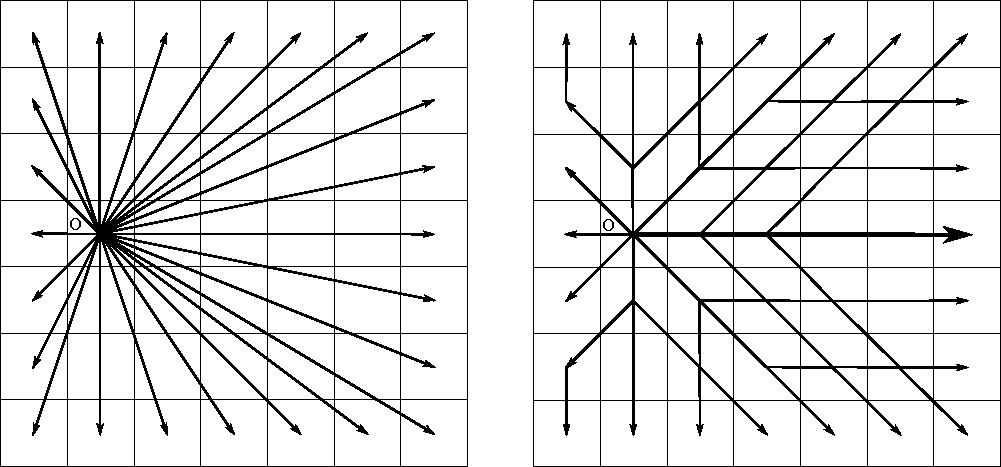
\includegraphics[scale=0.8]{img/grid.pdf} 
	\caption{Rays traced on a 7x7 pixel image from an observation point located at (4,2). On the left, the theoretical tracing of the rays, on the right the actual path of the rays on the pixels of the image.}
	\label{grid}
\end{figure}

For each ray, the pixels are traversed from the closest of the point O to the farthest. At each pixel, the vertical angle between the point O and the center of the pixel is calculated. If the angle is greater than the previous ones, the pixel is visible, otherwise it is not.

The height of the pixels corresponds to the sum of the elevation of the DTM and the height of the DSM if it is present. The height of the observation point O corresponds to the sum of the elevation of the DTM and the parameter $h1$ (height of the observer eye). The height of the DSM is never taken into account for the height of the observer (the observer does not climb the trees).

The figure \ref{ray_side} represents the calculation of a ray over 5 pixels. The pixel located on the observer's point (pixel 0) is always visible. The next pixel (1) is also visible, but pixel 2 is not visible because the target angle is smaller than for pixel 1, and so on.

\begin{figure}[H]
	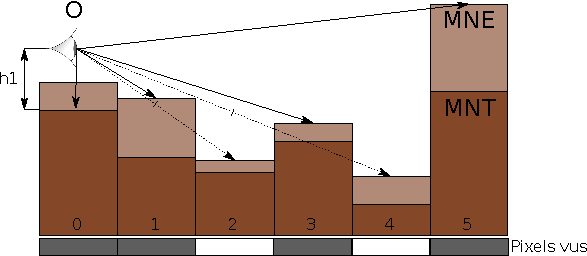
\includegraphics{img/ray_side-fr.pdf} 
	\caption{Side view of a ray tracing}
	\label{ray_side}
\end{figure}

The result of the calculation of the ray of the figure \ref{ray_side} is shown in the following figure (\ref {grid_result}). It corresponds to the pixels of the image which are traversed by the ray and which are visible from the observation point.

\begin{figure}[H]
	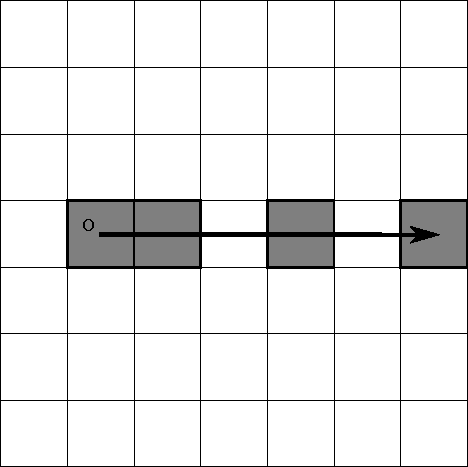
\includegraphics[scale=0.8]{img/grid_result.pdf} 
	\caption{Result in planimetric view of the ray calculated on the figure \ref{ray_side}. The pixels in gray are the visible pixels for this ray.}
	\label{grid_result}
\end{figure}

The complete result corresponds to the combination of the results for each ray.
As the pixels of the image can be traversed by different rays, a pixel is marked visible when it is visible by at least one of the rays passing through it.

\subsection{Reverse planimetric view}

The reverse mode inverts the observer and the observed. The viewshed is no longer the area visible from the point O, but the area that sees the point O. The point O is the observed point and the observer is positioned on all points of the image. Figure \ref{ray_side_inverse} shows the process for a given ray.

\begin{figure}[H]
	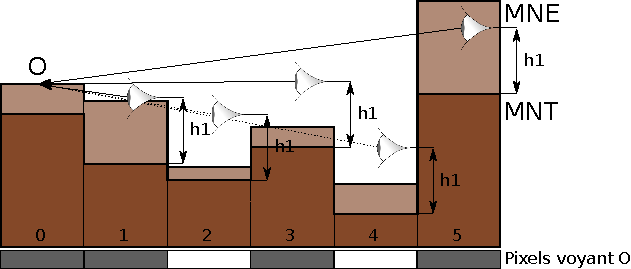
\includegraphics{img/ray_side_inverse-fr.pdf} 
	\caption{Side view of a ray tracing in reverse mode.}
	\label{ray_side_inverse}
\end{figure}

The result is identical in this example, but according to the configuration, it may be different in reverse mode.

\section{Tangential view}
\label{principles_tan}
For the tangential view, the principle of computation is close but has some differences. First, the scan of the image is not necessarily exhaustive. The number of calculated rays is no longer dependent on the size of the image but on the angular resolution parameter $\alpha$. By default, this parameter is set to 0.1 °. The number of calculated rays is 3600. Figure \ref{grid_tan} shows an example with an angular accuracy of 30°.

\begin{figure}[H]
	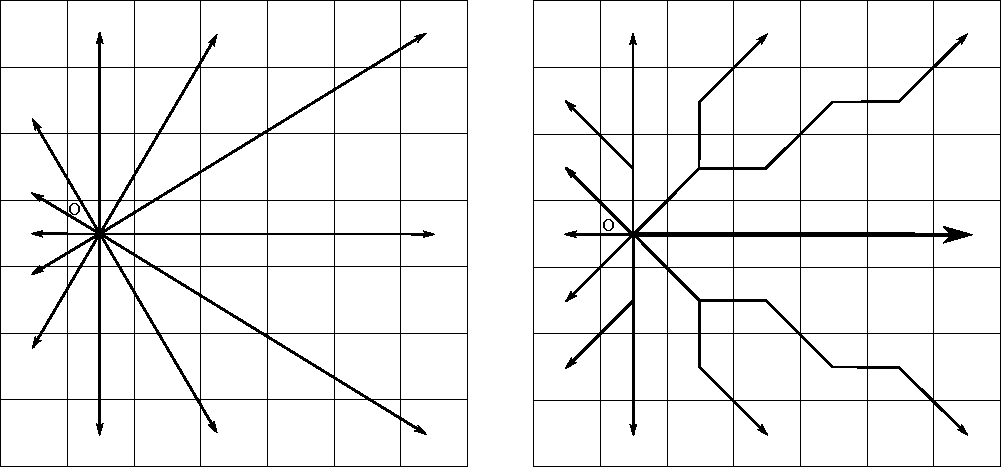
\includegraphics[scale=0.8]{img/grid_tan.pdf} 
	\caption{Rays traced on a 7x7 pixels image from an observation point located at (4,2). On the left, the theoretical tracing of the rays, on the right the actual path of the rays on the pixels of the image. The angular accuracy ($\alpha$) here is very coarse: 30°.}
	\label{grid_tan}
\end{figure}

In the calculation of each ray, additional processing must be performed to determine the angle height of each visible pixel (figure \ref{ray_side_tan}). The result is represented by the column to the right of the figure \ref{ray_side_tan} for an angular precision ($\alpha$) of 10°.

\begin{figure}[H]
	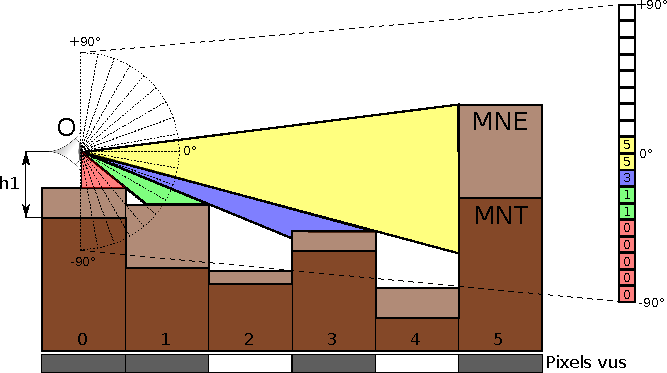
\includegraphics{img/ray_side_tan-fr.pdf} 
	\caption{Side view of ray tracing. Calculation of the angle heights of the visible pixels for the tangential view. The angular accuracy here is very coarse: 10°.}
	\label{ray_side_tan}
\end{figure}

The juxtaposition of the columns resulting from each ray forms the result of the tangential view. Figure \ref{grid_tan_result} shows the position of each ray calculated in the tangential view for an angular accuracy of 30°.

\begin{figure}[H]
	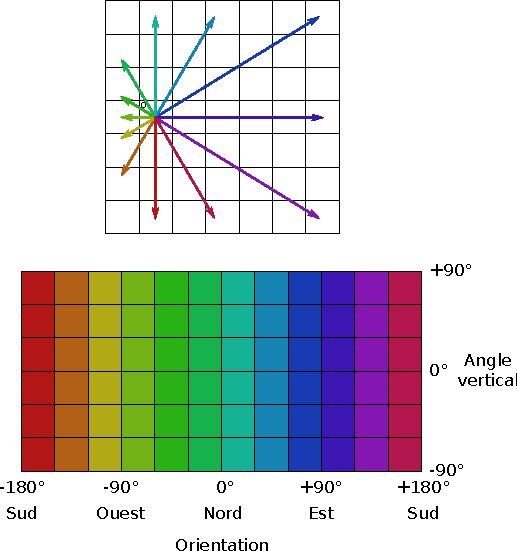
\includegraphics{img/grid_tan_result.pdf} 
	\caption{Position of each ray calculated in the tangential view. The angular accuracy here is very coarse: 30°.}
	\label{grid_tan_result}
\end{figure}

\section{Multiscale}
\label{multires}
The multiscale calculation can greatly speedup visibility processing. Indeed, the algorithmic complexity of a visibility calculation is proportional to the number of pixels of the image $n$. In multiscale, the complexity decreases to $log(n)$ as long as the resolutions evolve geometrically.

\begin{figure}[H]
	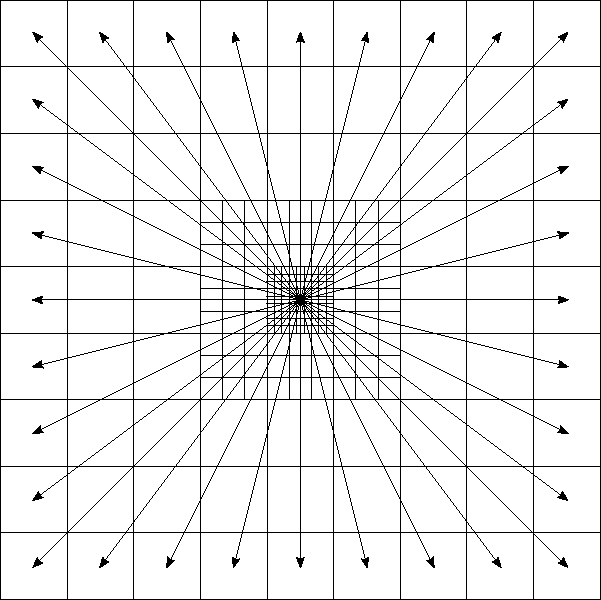
\includegraphics{img/grid_multi.pdf} 
	\caption{Ray tracing on a multiscale database of factor 3 with 3 resolutions}
	\label{grid_multi}
\end{figure}

In the example of figure \ref{grid_multi}, the number of calculated rays is 32 instead of 306 and the length of the rays in pixels is 11 instead of 41. The gain in computation time is approximately 35 while retaining the constraint of covering the whole space.


\section{Eyesight bounds}
\label{bounds}
For all visibility calculations integrated into PixScape, the eyesight can be restricted in the 3 dimensions (figures \ref{bounds_side} and \ref{bounds_2d}) by 6 parameters: the minimum distance ($d_{min}$) and maximum distance ($d_{max}$), the minimum vertical angle ($z_{min}$) and maximum vertical angle ($z_{max}$), and the horizontal angle by the orientation ($orien$) and the amplitude ($amp$). The angles are expressed in degrees in the interval [0-360] for the horizontal angles and [-90; +90] for the vertical angles. The distances are expressed in meters and are calculated in 2D on the plane (x, y).

\begin{figure}[H]
	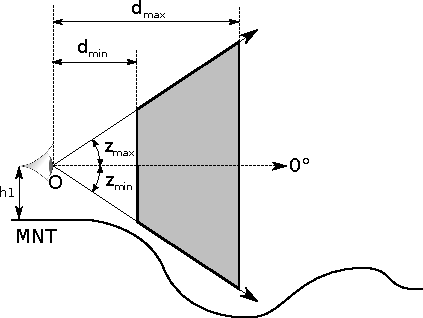
\includegraphics{img/bounds_side.pdf} 
	\caption{Side view of the eyesight bounds}
	\label{bounds_side}
\end{figure}

\begin{figure}[H]
	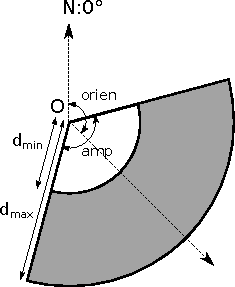
\includegraphics{img/bounds_2d.pdf} 
	\caption{Top view of the eyesight bounds}
	\label{bounds_2d}
\end{figure}


\chapter{Metrics description}
\label{metrics}
In this chapter, all the metrics available in PixScape are described. The \ref{metrics_tab} table lists all these metrics and what they support: support of planimetric and/or tangential views, support or not of land use and support of distance intervals.

\begin{table}[H]
	\begin{tabular}{|c|c|c|c|c|c|c|}
		\hline
		Metric & Name & Planimetric & Tangential & Without LU & With LU & Distance\\
		\hline
		A & Area & X & X & X & X & X\\
		\hline
		S & Shannon diversity index & X & X &  & X & X\\
		\hline
		AG & Aggregation index & X & X &  & X & \\
		\hline
		CONTAG & Contagion & X & X &  & X & \\
		\hline
		ED & Edge Density & X & X &  & X & \\
		\hline
		PD & Patch Density & X & X &  & X & \\
		\hline
		PMS & Patch Mean Size & X & X &  & X & \\
		\hline
		DIST & Distance distribution & X & X & X &  & \\
		\hline
		P & Perimeter & X &  & X &  & \\
		\hline
		C & Compactness & X &  & X &  & \\
		\hline
		FD & Fractal dimension & X &  & X &  & \\
		\hline
		SL & Skyline &  & X & X &  & X \\
		\hline
		SD & Shannon depth &  & X & X &  & \\
		\hline
		DL & Depth line &  & X & X &  & \\		
		\hline
	\end{tabular}
	\caption{List of metrics and their parameters}
	\label{metrics_tab}
\end{table}

\section{Common metrics}

\subsection{Area: A}
This metric measures the visible area in square meters for the planimetric view and in square degrees for the tangential view. The calculation may be restricted to certain categories of land use and for different distance intervals.

\subsection{Shannon diversity index: S}
This metric calculates the Shannon index on the parts of the visible area of each land use category. It is used to measure the diversity of the visible land use.

$$S = -\frac{1}{\ln n}\sum_{i=1}^{n}\frac{A_i}{A}\ln\left(\frac{A_i}{A}\right)$$

With $n$ the number of land use category, $A_i$ the visible area of the category $i$ and $A$ the total visible area. Areas are expressed in square meters for the planimetric view and in square degrees for the tangential view.

The project must contain the land use layer for using this metric.

\subsection{Aggregation index: AG}
This metric corresponds to the Aggregation index (AI) defined in Fragstat. In PixScape, the calculation of this metric is applied to the visible land use areas only.

$$AG = \sum_{i=1}^n \frac{A_i}{A} AG_i, AG_i = 100 \frac{g_{ii}}{\max g_{ii}}$$

With $g_{ii}$ the number of like adjacencies (joins) between pixels of landuse class $i$ based on the single-count method and $\max g_{ii}$ the theoretical maximum \textit{ie.} when the shape of the landuse class $i$ is a square.

The project must contain the land use layer for using this metric.

\subsection{Contagion: CONTAG}
This metric corresponds to the contagion index defined in Fragstat. In PixScape, the calculation of this metric is applied to the visible land use areas only.

$$ CONTAG = 100 \left[1+\dfrac{1}{2\ln m} \sum _{i=1}^{m}  \sum _{j=1}^{m}  p_i\dfrac{g_{ij}}{\sum _{k=1}^{m}g_{ik} }   \ln \left( p_i\dfrac{g_{ij}}{\sum _{k=1}^{m}g_{ik} }\right)  \right]$$

It corresponds to the probability of finding a pixel of the land use category $i$
next to a pixel of the category $j$.

The project must contain the land use layer for using this metric.

\subsection{Edge density: ED}
This metric corresponds to the Edge density (ED) defined in Fragstat. In PixScape, the calculation of this metric is applied to the visible land use areas only.

$$ED = \frac{E}{A} = \frac{1}{2} \sum_{i=1}^{n} ED_i, ED_i = \frac{E_i}{A}$$

With $E$ the number of edges and $A$ the total visible area in square meters for the planimetric view and in square degrees for the tangential view.

Edges at the border of the visible area are not counted.

The project must contain the land use layer for using this metric.

\subsection{Patch density: PD}
This metric corresponds to the Patch density (PD) defined in Fragstat. In PixScape, the calculation of this metric is applied to the visible land use areas only.

$$PD = \frac{p}{A} = \sum_{i=1}^{n} PD_i, PD_i = \frac{p_i}{A}$$

With $p_i$ the number of patches of the landuse category $i$ and $A$ the total visible area in square meters for the planimetric view and in square degrees for the tangential view.

The project must contain the land use layer for using this metric.

\subsection{Patch Mean Size: PMS}
This metric corresponds to the average size of a patch in square meters for the planimetric view and in square degrees for the tangential view. The calculation of this metric is applied to the visible land use areas only.

$$PMS = \frac{A}{p}, PMS_i = \frac{A_i}{p_i}$$

With $p_i$ the number of patches of the landuse category $i$ and $A$ the total visible area in square meters for the planimetric view and in square degrees for the tangential view.

The project must contain the land use layer for using this metric.

\subsection{Distance distribution: DIST}

The $DIST$ metric gives an overview of the distribution of the pixel distances visible from the observation point by four aggregation operators: sum, average, minimum and maximum.

The result of the metric is different between the tangential and planimetric view, the visible pixels being not distributed in the same way between the two views. Indeed, in planimetric, each pixel represents a surface on the ground in square meters, whereas in tangential view, each pixel represents a cone of the eyesight in square degrees.


\section{Planimetric metrics}

\subsection{Perimeter: P}

The metric P corresponds to the total perimeter of the viewshed, including the whole of contour both external and internal. The unit is in meters.


\subsection{Compactness: C}
This metric takes the compactness index applied to the whole viewshed such as:

$$C=\frac{P}{2\sqrt{\pi A}}$$

If $C=1$ the viewshed is compact \textit{ie.} a full disk. The more $C$ increases, the smaller the viewshed compactness is.


\subsection{Fractal dimension: FD}
This metric calculates the fractal dimension of the viewshed. The method used is the box counting.

The result is between 0 and 2. When $FD$ tends to 0 the viewshed is reduced to a point, when $FD$ tends to 2 the viewshed covers the space in a homogeneous way.

\section{Tangential metrics}

\subsection{Skyline: SL}

The $SL$ metric measures the more or less uneven aspect of the skyline. It is calculated as the ratio of the length of the skyline ($l_h$) to a flat horizon line ($L = 360\deg$). The lengths are expressed in degrees.

$$SL=\frac{l_h}{L}$$

$SL$ is close to 1 when the horizon is planar, and highest (unbounded) in the case of a very jagged skyline.

\subsection{Shannon depth: SD}
The $SD$ metric measures the greater or lesser variation of sight lengths.

It corresponds to the standardized Shannon index applied to the distribution of the view depths grouped into $m$ classes. The distance classes are defined by a geometric sequence: less than 10m, 10 to 100m, 100m to 1km, 1km to 10km, and more than 10km.

$$SD = -\frac{1}{\ln m}\sum_{i=1}^{m}\frac{nd_i}{n}\ln\left(\frac{nd_i}{n}\right)$$

with $nd_i$ the number of rays with a maximal length inside the class $i$ and $n$ the total number of rays calculated in the tangential view.

This metric is 0 when all lengths are inside the same class, the view depth is homogeneous. Conversely, $SD$ is 1 when the ray lengths are equally distributed on all classes, which represents a large variation of view depth.


\subsection{Depth line: DL}
The $DL$ metric also measures the greater or lesser variation of the depths of view but without distance classes a priori as $SD$.

This metric requires the construction of a polygon on the plane (x, y) grouping the visible points furthest from the observation point for each ray being traced. The $DL$ metric is defined as the compactness index of this polygon:

$$DL=\frac{p}{2\sqrt{\pi a}}$$

where $p$ and $a$ represent respectively the perimeter and the area of the polygon. 

This metric gives a minimum value of 1 in the case of equal view depths (the polygon is a circle), and high (unbounded) values in the case of strong variations in view depths.


\chapter{Performance tuning}
\label{perf}

\section{Parallelism to speed up execution}
\label{parallelism}
To reduce visibility calculation execution time, PixScape implements 3 parallelization methods: thread based for a single computer, CUDA to use Graphic Processor Unit (GPU) acceleration, and MPI for computer clusters.

The table \ref{perf_table} shows the execution times to calculate 10000 views according to the type of view (planimetric or tangential), the size of the DTM in million pixels and the parallelization: 1 core (without parallelization), 4 cores, 16 cores and GPU (NVidia Tesla K40 graphics card).

\begin{table}[htbp]
	
	\begin{tabular}{|l|r|r|r|r|r|}
		\hline
		Type & \multicolumn{1}{l|}{Size} & \multicolumn{1}{l|}{1 core} & \multicolumn{1}{l|}{4 cores} & \multicolumn{1}{l|}{16 cores} & \multicolumn{1}{l|}{GPU} \\ \hline
		\multicolumn{ 1}{|c|}{Planimetric} & 1 M & 9,8 & 2,5 & 0,7 & 0,6 \\ \cline{ 2- 6}
		\multicolumn{ 1}{|l|}{} & 9 M & 103,0 & 26,0 & 6,7 & 1,8 \\ \cline{ 2- 6}
		\multicolumn{ 1}{|l|}{} & 100 M & 1168,0 & 376,0 & 83,0 & 13,2 \\ \hline
		\multicolumn{ 1}{|c|}{Tangential} & 1 M & 36,0 & 9,8 & 2,7 & 0,8 \\ \cline{ 2- 6}
		\multicolumn{ 1}{|l|}{} & 9 M & 113,0 & 28,8 & 8,0 & 2,2 \\ \cline{ 2- 6}
		\multicolumn{ 1}{|l|}{} & 100 M & 357,0 & 91,0 & 24,7 & 6,3 \\ \hline
	\end{tabular}
	\caption{Average time in minutes to calculate 10000 views.}
	\label{perf_table}
\end{table}


\subsection{One computer : threads}
\label{thread}
Multi-threaded parallelization accelerates computation time on a single machine containing multiple cores or processors. If your computer has more than one core (most of them), you can take advantage of multi-threading to speed up your calculations with PixScape. The execution time is approximately inversely proportional to the number of cores used. 

This parallelism method can be used in GUI and CLI.

\subsubsection{Graphical user interface}
The "Preferences" window accessible from the File menu allows you to set the number of cores used by PixScape. It is set by default to the number of cores of the computer minus 1. After changing the number of cores used by PixScape, it is better to restart PixScape to be sure that the change is taken into account.

\subsubsection{Command line interface}
On the command line, you have to define the number of cores (or processors) that PixScape can use with the \verb|-proc| option :
\begin{Verbatim}
java -jar pixscape-1.2.jar -proc 8 --project path2myproject/myproject.xml ...
\end{Verbatim}
By default, CLI uses the number of processors defined in the preferences window of the GUI.

By increasing the number of cores used by PixScape, you increase the memory size used by PixScape at the same time.


\subsection{Graphics card : CUDA}
\label{cuda}
This parallelism method makes it possible to carry out the visibility calculations on the graphics card instead of the processor. Runtime gains can be significant for Nvidia Tesla graphics cards, designed for high-performance computing (see \nameref{perf_table}). However, not all metrics are optimized for the GPU. Metrics A and S are the only ones to be optimized. If you use other metrics, the time savings will be minimal or non-existent.

To use GPU acceleration, you need a Nvidia graphics card that supports CUDA and CUDA version 6.5 installed. 

If PixScape fails to use the GPU, the calculations will be automatically switched to the processor.

This parallelism method can be used in GUI and CLI.

\subsubsection{Graphical user interface}

The activation of the GPU acceleration can be done from the Options window (see \nameref{options}).

In graphical interface, PixScape can only use one graphics card, if your computer contains several graphic cards, PixScape can use them in parallel but only on the command line.

\subsubsection{Command line interface}
At the command line, the \verb|-cuda| option activates the use of the GPU. It is also necessary to give the number of graphics cards to use.

\begin{Verbatim}
java -jar pixscape-1.2.jar -cuda 1 --project path2myproject/myproject.xml ...
\end{Verbatim}
In the example above, PixScape use one graphics card for visibility calculations. If your computer contains several graphics cards, it is possible to increase the parameter to use them in parallel and decrease the time of execution accordingly.


\subsection{Computer cluster : mpi}
PixScape can also be used on computing clusters supporting Java with OpenMPI. This parallelism method is only available on the command line.

Exemple :
\begin{Verbatim}
mpirun java -jar pixscape-1.2.jar -mpi --project path2myproject/myproject.xml ...
\end{Verbatim}
Only some commands can be used in the MPI environment: \verb|--planmetric|, \verb|--tanmetric|, \verb|--landmod|


\section{Memory management}
\label{memory}
By default, the amount of memory available for PixScape is system dependent.  It can vary from 128 Mb to several Gb.  In most cases, PixScape will run normally.  But if you have a large project, some processes would be slow or even crash due to memory limitation.

Also, if you use thread-based parallelism (\nameref{thread}), PixScape will need more memory for each core used.

In all cases, if PixScape execution terminates with OutOfMemoryError
or GC overhead, you need to increase memory allocated to PixScape.


\subsection{Graphical user interface}
The memory allocated for PixScape can be changed in the "Preferences" window on the File / Preferences menu. After changing this setting, PixScape must be restarted to take the new memory size into account.

In GUI, PixScape needs more memory than command line because of the layers display. If you are too limited in RAM, you can run the calculations on command line interface to reduce PixScape memory requirements (see \nameref {cli}).

\subsection{Command line interface}
To define manually the maximum amount of memory allocated to PixScape, use Java option \verb|-Xmx|:

\begin{Verbatim}
java -Xmx4g -jar pixscape-1.2.jar ... # 4Gb allocated
java -Xmx1500m -jar pixscape-1.2.jar ... # 1500 Mb -> 1.5Gb allocated
\end{Verbatim}

If you cannot allocate more than 1Gb or 1.5Gb and your computer has more memory available, you have
probably a 32-bit version of Java, which is limited to less than 2Gb of memory.  Check your Java version:
\begin{Verbatim}
java -version
\end{Verbatim}
If it is a 32-bit version, install a 64-bit Java version to handle all your computer memory.


%\section{Multi-résolution}

\end{document}
